%% This template can be used to write a paper for
%% Computer Physics Communications using LaTeX.
%% For authors who want to write a computer program description,
%% an example Program Summary is included that only has to be
%% completed and which will give the correct layout in the
%% preprint and the journal.
%% The `elsarticle' style is used and more information on this style
%% can be found at 
%% http://www.elsevier.com/wps/find/authorsview.authors/elsarticle.
%%
%%
%% \documentclass[preprint,12pt]{elsarticle}

%% Use the option review to obtain double line spacing
%% \documentclass[preprint,review,12pt]{elsarticle}

%% Use the options 1p,twocolumn; 3p; 3p,twocolumn; 5p; or 5p,twocolumn
%% for a journal layout:
%% \documentclass[final,1p,times]{elsarticle}
%% \documentclass[final,1p,times,twocolumn]{elsarticle}
%% \documentclass[final,3p,times]{elsarticle}
%% \documentclass[final,3p,times,twocolumn]{elsarticle}
%% \documentclass[final,5p,times]{elsarticle}
\documentclass[final,5p,times,twocolumn]{elsarticle}

%% if you use PostScript figures in your article
%% use the graphics package for simple commands
%% \usepackage{graphics}
%% or use the graphicx package for more complicated commands
%% \usepackage{graphicx}
%% or use the epsfig package if you prefer to use the old commands
%% \usepackage{epsfig}

%% The amssymb package provides various useful mathematical symbols
\usepackage{amssymb}
\usepackage{fancyvrb}
\usepackage[T1]{fontenc}
\PassOptionsToPackage{hyphens}{url}\usepackage{hyperref}
%% The amsthm package provides extended theorem environments
%% \usepackage{amsthm}

%% The lineno packages adds line numbers. Start line numbering with

%% \begin{linenumbers}, end it with \end{linenumbers}. Or switch it on
%% for the whole article with \linenumbers after \end{frontmatter}.
%% \usepackage{lineno}

%% natbib.sty is loaded by default. However, natbib options can be
%% provided with \biboptions{...} command. Following options are
%% valid:

%%   round  -  round parentheses are used (default)
%%   square -  square brackets are used   [option]
%%   curly  -  curly braces are used      {option}
%%   angle  -  angle brackets are used    <option>
%%   semicolon  -  multiple citations separated by semi-colon
%%   colon  - same as semicolon, an earlier confusion
%%   comma  -  separated by comma
%%   numbers-  selects numerical citations
%%   super  -  numerical citations as superscripts
%%   sort   -  sorts multiple citations according to order in ref. list
%%   sort&compress   -  like sort, but also compresses numerical citations
%%   compress - compres ses without sorting
%%
%% \biboptions{comma,round}

% \biboptions{}

%% This list environment is used for the references in the
%% Program Summary
%%
\newcounter{bla}
\newenvironment{refnummer}{%
\list{[\arabic{bla}]}%
{\usecounter{bla}%
 \setlength{\itemindent}{0pt}%
 \setlength{\topsep}{0pt}%
 \setlength{\itemsep}{0pt}%
 \setlength{\labelsep}{2pt}%
 \setlength{\listparindent}{0pt}%
 \settowidth{\labelwidth}{[9]}%
 \setlength{\leftmargin}{\labelwidth}%
 \addtolength{\leftmargin}{\labelsep}%
 \setlength{\rightmargin}{0pt}}}
 {\endlist}

\journal{Computer Physics Communications}

\begin{document}

\begin{frontmatter}

%% Title, authors and addresses

%% use the tnoteref command within \title for footnotes;
%% use the tnotetext command for the associated footnote;
%% use the fnref command within \author or \address for footnotes;
%% use the fntext command for the associated footnote;
%% use the corref command within \author for corresponding author footnotes;
%% use the cortext command for the associated footnote;
%% use the ead command for the email address,
%% and the form \ead[url] for the home page:
%%
%% \title{Title\tnoteref{label1}}
%% \tnotetext[label1]{}
%% \author{Name\corref{cor1}\fnref{label2}}
%% \ead{email address}
%% \ead[url]{home page}
%% \fntext[label2]{}
%% \cortext[cor1]{}
%% \address{Address\fnref{label3}}
%% \fntext[label3]{}

\title{Pyg4ometry: a python library for the creation of Monte Carlo radiation transport physical geometries}

%% use optional labels to link authors explicitly to addresses:
%% \author[label1,label2]{<author name>}
%% \address[label1]{<address>}
%% \address[label2]{<address>}

\author[a]{Stewart T. Boogert\corref{author}}
\author[a]{Andrey Abramov}
\author[a]{Laurence Nevay}
\author[a]{William Shields}
\author[a]{Stuart Walker}

\cortext[author] {Corresponding author.\\\textit{E-mail address:} stewart.boogert@rhul.ac.uk}
\address[a]{John Adams Institute at Royal Holloway, Department of Physics, Royal Holloway, Egham, TW20 0EX, Surrey, UK}

\begin{abstract}
\end{abstract}

\begin{keyword}
%% keywords here, in the form: keyword \sep keyword
Geant; Monte Carlo; Particle; Transport; Geometry; 

\end{keyword}

\end{frontmatter}

%%
%% Start line numbering here if you want
%%
% \linenumbers

% Computer program descriptions should contain the following
% PROGRAM SUMMARY.

{\bf PROGRAM SUMMARY/NEW VERSION PROGRAM SUMMARY}
  %Delete as appropriate.

\begin{small}
\noindent
{\em Program Title: pyg4ometry }                                         		\\
{\em Licensing provisions(please choose one): GPLv3 }			\\
{\em Programming language: python, C/C++}                         		\\

{\em Supplementary material:}                                 				\\
  % Fill in if necessary, otherwise leave out.
{\em Journal reference of previous version:}                  			\\
  %Only required for a New Version summary, otherwise leave out.
{\em Does the new version supersede the previous version?:}   	\\
  %Only required for a New Version summary, otherwise leave out.
{\em Reasons for the new version:}							\\
  %Only required for a New Version summary, otherwise leave out.
{\em Summary of revisions:}*								\\
  %Only required for a New Version summary, otherwise leave out.

{\em Nature of problem(approx. 50-250 words):}\\
Creating computer readable geometry descriptions for Monte Carlo radiation transport codes is a time consuming and error prone task.  \\
{\em Solution method(approx. 50-250 words):}\\
  %Describe the method solution here.
{\em Additional comments including Restrictions and Unusual features (approx. 50-250 words):}\\
  %Provide any additional comments here.
   \\

\begin{thebibliography}{0}
\bibitem{1}Reference 1         % This list should only contain those items referenced in the                 
\bibitem{2}Reference 2         % Program Summary section.   
\bibitem{3}Reference 3         % Type references in text as [1], [2], etc.
                               % This list is different from the bibliography at the end of 
                               % the Long Write-Up.
\end{thebibliography}
* Items marked with an asterisk are only required for new versions
of programs previously published in the CPC Program Library.\\
\end{small}


%% main text
\section{Introduction} \label{sec:introduction}
There are numerous different software codes to simulate the passage of particles through material, so called radiation transport (RT) programmes, these 
include MCNP \cite{Mcnp_Werner}, FLUKA \cite{Fluka_Ferrari,Fluka_Bohlen}, Geant3 \cite{Geant3_Brun} and Geant4 \cite{Geant4_Agostinelli}. 
All these codes are based on the Monte Carlo technique but each code either has a particular specialism or target user community.  RT Monte Carlo (RTMC) simulations 
have diverse uses, shielding calculations for radiological protection, detector performance, medical imaging and therapy and space radiation environment 
simulation are some examples. A fundamental requirement of all of the codes is to supply a computer readable description of the physical geometry that 
the particles are passing through.  The creation of geometry files is typically a very time consuming activity and the simulation validity and performance is directly 
dependent on the quality of the geometry. The requirement of a geometry system that allows the conversion between files prepared for different codes will 
enable cross checks of the physics processes in different particle transport codes. Parallel to the creation of geometry files for RT programs, usually computer assisted 
design (CAD) files exist for systems which need to be simulated in RT programmes. The fundamental geometric representations in CAD files is typically not 
amenable for RT programmes.  For these reasons it is advantageous to create a software tool that allows particle transport code users to rapidly develop 
geometry files, convert between common RT programme geometry formats and finally import CAD models. 

This paper describes such geometry creation and conversion package called {\em pyg4ometry}, implemented in {\em Python} and internally based on the Geant4 geometry 
description. The main features of  {\em pyg4ometry} are a python scripting API to rapidly design parametrised geometry, conversion to and from  FLUKA geometry 
descriptions, conversion from CAD formats  (STEP and IGES) based on FreeCAD \cite{FreeCAD} OpenCascade \cite{OpenCASCADE} and powerful geometry 
visualisation tools based on VTK \cite{VTK4}. The origin of pyg4ometry was a set of utilities to prepare geometry for an accelerator beam line simulation based on Geant4 
called BDSIM. Accelerator physicists like specialists in other areas need a tool to quickly simulate beam losses, and the subsequent interaction of the charged particle 
beam with the accelerator material.

There are existing codes that have functionality similar to pyg4ometry. Tools exist to convert CAD files to GDML, open source examples are GUIMesh \cite{GUIMesh_Pinto}, 
commercial products include ESABASE2 \cite{ESABASE2} and FASTRAD \cite{FASTRAD}. 
CAD software can export data to STL. The existent set of software does not provide a complete set of tools to efficiently create complex geometries.   

\section{Geometric descriptions} \label{sec:geometric}
Central to description of a geometric description of a system is how a solid is defined in three dimensions. There are numerous different ways to describe a
geometry and these are described briefly in the following sections.  

\subsection{Constructive solid geometry (CSG)}
Constructive solid geometry uses boolean operations (subtraction, intersection and union) between simple solids shapes (cube, cylinder, sphere etc) to model complex 
surfaces which represent a solid. Typically simple finite or infinite solids are combined with operations, such as union, intersection and difference to model more 
complex solids. FLUKA uses CSG to model solids.

\subsection{Boundary representation (BREP)}
Boundary representation consists of two parts, topology and geometry. Topological elements are faces, edges and vertices. No current RT applications use native 
file formats employed by CAD systems. The conversion of CAD BREP formats for loading in RT applications is typically performed via a tessellated format, although it 
is possible to decompose BREP descriptions to simple half-spaces and solids as used in CSG descriptions. 

\subsection{Tessellated polygons}
Solid volumes can be defined using triangular, quadrilateral or tetrahedral meshes. Numerous formats exist to describe meshes, the ubiquitous being STL and more 
modern variants being PLY, OBJ, etc. For solids with curved faces a tessellated mesh will always give an approximate description. As the mesh deviation distance from the 
solid decreases the number of polygons increases and hence the memory consumption and execution time of the RTMC. 

\subsection{Geant4 geometery}
Geant4 geometry description is a mixture of BREP, CSG and tessellated concepts. Geant4 includes XX fundamental solids, although it does not store a sense 
of topology present in traditional CAD BREP systems. One of the fundamental solids is a {\em TessellatedSolid} which can used to represent STL or PLY files. 
Geant4 also provides the ability to perform boolean operations on these primitive solids. The richest and most flexible geometry description is currently used by
Geant4. Not only do solid objects need to be defined but also placed in a world coordinate system. Geant4 has two concepts which facilitate this {\it Logical Volumes} 
and {\it Physical Volumes}. A Logical Volume is a region of space  that is defined by an outer solid but also other attributes like material, magnetic field and zero or 
more physical {\it daughter} volumes. A Physical Volume is a placement (or instance) of a Logical Volume.   

\subsection{Geant Detector Mark-up Language} 
To exchange geometry descriptions Geant Detector Mark-up Language (GDML) was developed. Geant4 and ROOT can read and write GDML format and it is commonly
used as an exchange format for Geant4 geometries. 
\begin{table}[hbt!]
\centering
\begin{tabular}{|l|l|l|} \hline
GDML tag 		& Child tags				& pyg4ometry class 				\\ \hline
Define 			& Constant				& gdml.Constant				\\
				& Variable					& gdml.Variable					\\
				& Quantity					& gdml.Quantity				\\
				& Expression 				& gdml.Expression				\\
				& Position					& gdml.Position					\\
				& Rotation					& gdml.Rotation				\\
				& Scale					& gdml.Scale					\\
				& Matrix					& gdml.Matrix					\\ \hline
Materials 			& Element					& geant4.Element				\\
				& Isotope					& geant4.Isotope				\\
				& Material					& geant4.Material				\\ \hline
Solid  			& Box					& geant4.solid.Box				\\
	  			& Tube					& geant4.solid.Tubs				\\
	  			& CutTube				& geant4.solid.CutTubs			\\
	  			& Cone					& geant4.solid.Cons				\\
	  			& Para					& geant4.solid.Para				\\
	  			& Trd					& geant4.solid.Trd				\\
	  			& Trap					& geant4.solid.Trap				\\
	  			& Sphere					& geant4.solid.Sphere			\\
	  			& Orb					& geant4.solid.Orb				\\
	  			& Torus					& geant4.solid.Torus				\\
	  			& Polycone				& geant4.solid.Polycone			\\
	  			& GenericPolycone			& geant4.solid.GenericPolycone	\\
	  			& Polyhedra				& geant4.solid.Polyhedra			\\
	  			& Eltube					& geant4.solid.EllipticalTube		\\
	  			& Ellipsoid					& geant4.solid.Ellipsoid			\\
	  			& Elcone					& geant4.solid.EllipticalCone		\\
				& Paraboloid				& geant4.solid.Paraboloid			\\
				& Hype					& geant4.solid.Hyperboloid		\\
				& Tet						& geant4.solid.Tet				\\
				& Xtru					& geant4.solid.ExtrudedSolid		\\
				& TwistedBox				& geant4.solid.TwistedBox		\\
				& TwistedTtap				& geant4.solid.TwistedTrap		\\
				& TwistedTrd				& geant4.solid.TwistedTrd 		\\
				& TwistedTube				& geant4.solid.TwistedTube		\\
				& Arb8					& geant4.solid.GenericTrap		\\
				& Tessellated				& geant4.solid.TessellatedSolid 	\\
				& Union					& geant4.solid.Union				\\
				& Subtraction				& geant4.solid.Subtraction			\\
				& Intersection				& geant4.solid.Intersection 		\\
				& MultiUnion				& geant4.solid.MultiUnion 			\\
				& ScaledSolid				& geant4.solid.ScaledSolid		\\				
	  			& OpticalSurface			& geant4.solid.OpticalSurface		\\ \hline
Structure			& Volume					& geant4.LogicalVolume			\\
				& Assembly				& geant4.AssemblyVolume 		\\
				& PhysVol					& geant4.PhysicalVolume			\\ 
				& ReplicaVol				& geant4.ReplicaVolume			\\ 
				& ParaVol					& geant4.ParameterisedVolume	\\ 
				& DivisionVol				& geant4.DivisionVolume			\\
				& SkinSurface				& geant4.SkinSurface			\\ 
				& BorderSurface			& geant4.BorderSurface			\\ \hline

\end{tabular}
\caption{GDML tags and corresponding pyg4ometry classes.}
\end{table}

\section{pyg4ometry design and layout}
The core of {\em pyg4ometry} consists of python classes that mimic Geant4 solids, logical, physical volume objects, GDML parameters and material classes.
The constructors of the python classes are kept as close to the original Geant4 C++ implementation so that {\it pyg4ometry} users do not have to learn 
a new API. Geometry construction in python proceeds in a way which is very similar to geometry construction in Geant4. A user relatively familiar with Geant4
should be able to start creating geometry in pyg4ometry immediately. In the following sections novel or important developments in {\it pyg4ometry} are described.  

\begin{figure*}[hbt]
  \normalsize
  \centering
  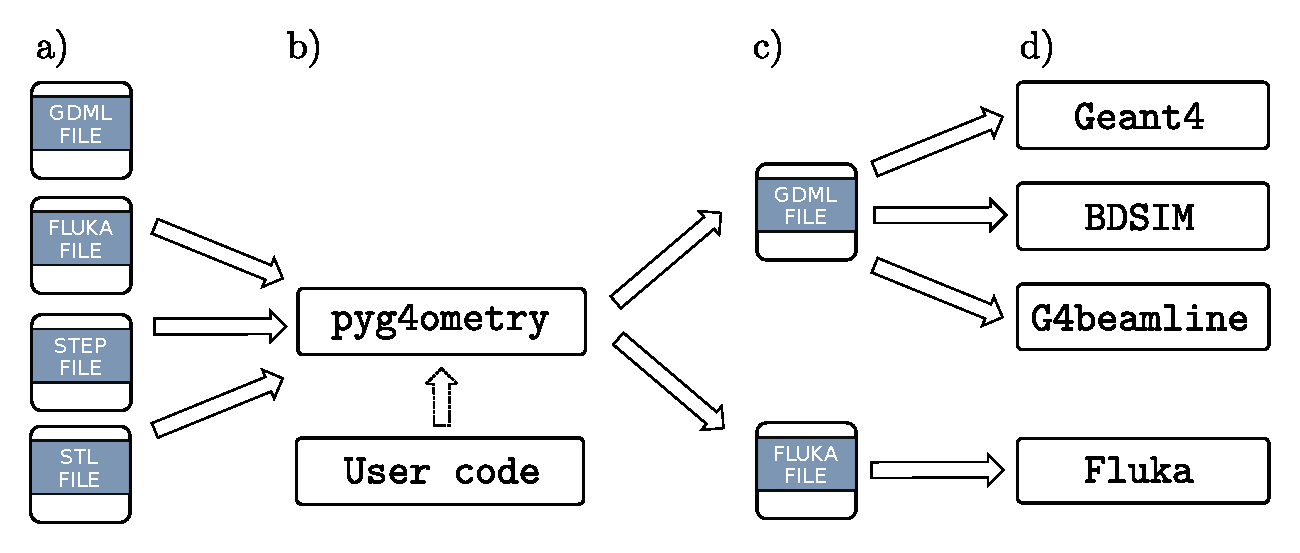
\includegraphics[width=0.7\textwidth]{./diagrams/workflow.pdf}
  \caption{\label{fig:workflow}Pyg4ometry geometry conversion workflow.}
\end{figure*}

    
\subsection{Expression evaluation}
In GDML symbolic expressions can be used to parametrise solids and their placement. These expressions are evaluated when the GDML is loaded into Geant4. 
In order to fully replicate the functionality of GDML an expression engine was implemented using ANTLR. GDML allows for the definition and assignment of 
variables. GDML expressions are not much more complicated than binary operators $+, -, \times, /$ and common trigonometric and special functions $\sin, \cos, \tan$ etc. 
The AST terminates on either expressions which evaluate to numbers or GDML variables. Internally all classes use GDML expressions and not floating point numbers. 
Storing internal data as expressions allows for deferred evaluation (or re-evaluation) of solid parameters and placements. This allows a user to update variables whilst
defining geometry and the expression engine will update all internal values.  
 
\subsection{Replica, division, parametrised and looped volumes}
A powerful feature of Geant4 and hence GDML is the ability to either repeat, divide or parametrise geometry. The create multiple replicas of a volume in a cartesian, cylindrical or 
spherical grid is known as a ReplicaVolume. Currently GDML loops are not supported by pyg4ometry and will be implemented in a future release. 

\subsection{Internal data representation} 
The internal data representation follows closely the structure of GDML. A \verb|Registry| class aggregates python ordered dictionaries that are  used to store the main 
elements of a GDML file. As a user specifies geometry the registry is updated. When a user is finished with the geometry, the registry is written to disk as a GDML file.
\verb|Registry| instances can be aggregated to form a composite geometry or volumes can be removed and added.   
  
\subsection{Input and output} 
For each input format available in pyg4ometry a dedicated {\it Reader} class is implemented, so \verb|gdml.Reader|, \verb|stl.Reader|, \verb|fluka.Reader| 
and \verb|freecad.Reader|. Each reader constructs the appropriate Geant4 classes and provides a registry which can be used or manipulated by the user. 
Output consists of taking the registry and writing the appropriate GDML.

\subsection{Tessellation of solids (meshing)}
For each Geant4 primitive solid a triangular tessellated Vertex-Face mesh is generated and cached. This mesh is then used to determine the extent of placed instances of 
geometry (physical volumes) and meshes for CSG derived solids. CSG mesh calculations are performed using a BSP tree technique. Triangular meshes based
on CSG operations involving curved surfaces often contain large numbers of thin triangles. Before meshes are visualised or written to disk various algorithms from 
TetGEN can be employed to give the meshes more desirable features. 

\subsection{Volume bounding} 
If a user is creating a placing multiple {\em daughter} volumes within a {\em mother} volume then it is the users responsibility to create a solid which fully encompasses the 
daughter volumes. Overlaps between daughter volumes and the mother can be detected, but it is desirable to have a mother volume shape that efficiently holds all of its daughters. 
 
\subsection{Visualisation}
A  geometry hierarchy can be viewed using the popular Visualisation Toolkit (VTK). No separate scene graph is required as the Geant4 volume hierarchy is sufficient 
to place the meshes associated with each physical volume. A daughter volume is placed within a logical volume with a rotation $\mathbf{R}$, scale $\mathbf{S}$ and 
translation $\mathbf{T}$.

\begin{figure}[htbp]
\begin{center}
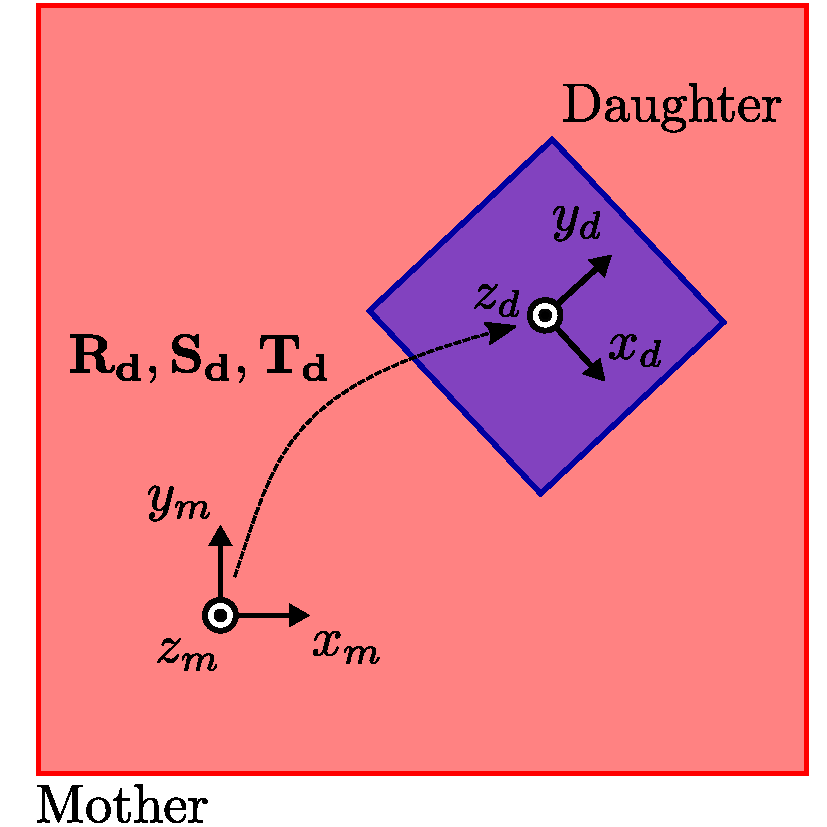
\includegraphics[width=5cm]{./diagrams/lvToPv.pdf}
\caption{Placement of physical volume inside a logical volume}
\label{fig:lvToPv}
\end{center}
\end{figure} 

\begin{eqnarray}
\mathbf{M}	  	& = & \mathbf{M}_m \mathbf{M}_d  = \mathbf{S}_m \mathbf{R}_m  \mathbf{S}_d \mathbf{R}_d\\
\mathbf{T}	 		& = & \mathbf{M}_m \mathbf{T}_d + \mathbf{T}_m= \mathbf{S}_m \mathbf{R}_m \mathbf{T}_d + \mathbf{T}_m,
\end{eqnarray}
where the subscript $p$ indicates parent volume and $d$ indicates daughter volume.

The python version of Geant4's physical volume is also used to store visualisation attributes like the solids 
color, surface or wireframe representation and visibility. Overlaps detected in the discretised mesh geometry can be displayed separately to allow a user to remove
the potential overlaps. This is dependent on the accuracy of the mesh generated and is a particular problem with meshes based on curved surfaces.    

\subsection{Adding properties to volumes}
A pure geometry description is an insufficient description for a RT simulation. Often other attributes need to be assigned for example material definition, magnetic field or  
optical surface properties.  

\subsection{Overlap detection}
All RT transport codes can not handle spatial overlap between two geometric objects and likely are to have ill defined behaviour when tracking particles  
through such a situation.  A key feature of pyg4ometry is the detection of potential overlaps efficiently, it does this by performing a CSG intersection between solid instances 
and determining if the resulting mesh is empty. Generally the overlap detection algorithm proceeds as 

{\small 
\begin{verbatim}
Overlap detection
\end{verbatim}
} 

For a logical volume with $n_{\rm daughters}$ physical volumes, assuming meshes for solids with average number of vertices $n$, clearly this algorithm has complexity $\sim \mathcal{O}(n^2 n_{\rm daughters})$. This might seem like a prohibitive computational cost, but worth it considering the potential waste if small overlaps are present in the final 
RT simulation. This algorithm clearly favours geometry descriptions which have a high degree of logical volume reuse. Due to the discrete nature of triangular meshes it is not possible to have perfect detection of overlaps, especially when curved surfaces are considered. 
 \begin{figure}[htbp]
\begin{center}
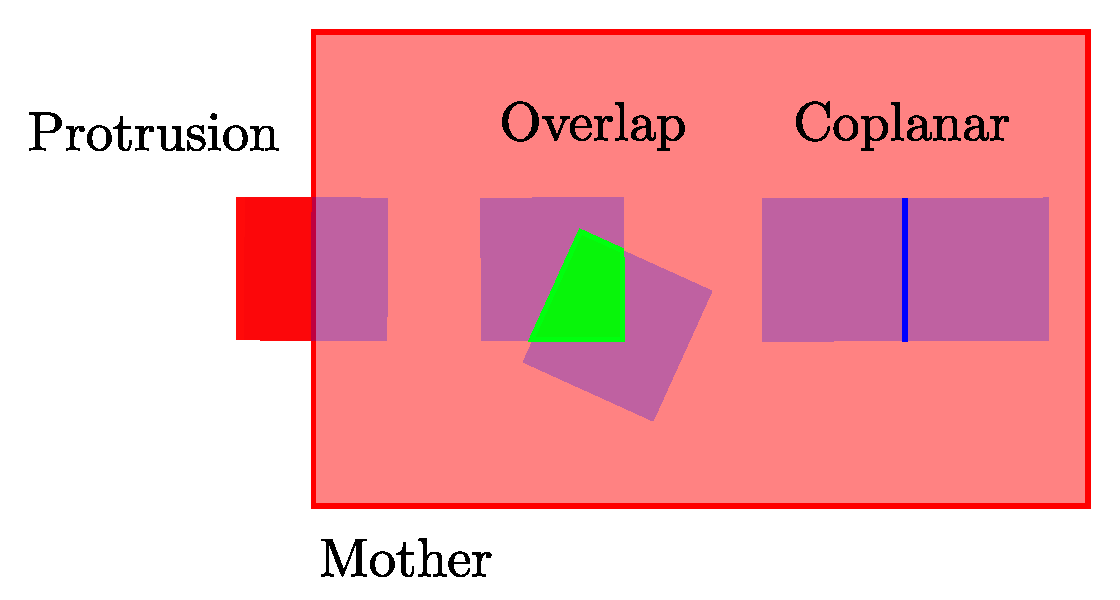
\includegraphics[width=8cm]{./diagrams/overlap.pdf}
\caption{Placement of physical volume inside a logical volume}
\label{fig:lvToPv}
\end{center}
\end{figure} 

\subsection{Graphical user interface}
A basic Qt based graphical user interface is also available with pyg4ometry. If a model has a large number of volumes defined in a hierarchical tree structure, it is cumbersome for the user to find the logical or physical volume.    

\section{Rapid geometry modelling}
Given the python scripting interface, expression  and tessellation engines. It is possible for a user to rapidly specify the geometrical layout of the RT problem, vary 
the parameters of the geometry and visualise the geometry. Finally when the desired result without geometry overlaps is finalised a GDML file can be output
from the internal memory representation. 

{\small
\begin{verbatim}
import pyg4ometry.gdml as gd
import pyg4ometry.geant4 as g4
import pyg4ometry.visualisation as vi

# create empty data storage structure
reg = g4.Registry()

# expressions 
wx = gd.Constant("wx","100",reg)
wy = gd.Constant("wy","100",reg)
wz = gd.Constant("wz","100",reg)

bx = gd.Constant("wx","10",reg)
by = gd.Constant("wy","10",reg)
bz = gd.Constant("wz","10",reg)

# materials
bm = g4.Material("G4_Galactic") 
wm = g4.Material("G4_Iron") 

# solids
wb = g4.solid.Box("wb",wx,wy,wz,reg)
b  = g4.solid.Box("b",bx,by,bz)

# structure 
wl = g4.LogicalVolume(wb, wm, "wl", reg)
bl = g4.LogicalVolume(b, bm, "b", reg)
bp1 = g4.PhysicalVolume([0,0,0],[0,0,0], 
                        bl, "b_pv1", wl) 
bp2 = g4.PhysicalVolume([0,0,0],[-2*bx,0,0], 
                        bl, "b_pv2", wl)  
bp3 = g4.PhysicalVolume([0,0,0],[2*bx,0,0], 
                        bl, "b_pv3", wl) 
                        
# gdml output
w = gd.Writer()
w.write(reg,"output.gdml")

# visualisation 
v = vi.VtkViewer()
v.addLogicalVolume(wl)
v.view()
\end{verbatim}
}

An example of the VTK output for code listing XXX is shown in Figure~\ref{fig:rapidModellingExample}.
\begin{figure}[htbp]
\begin{center}
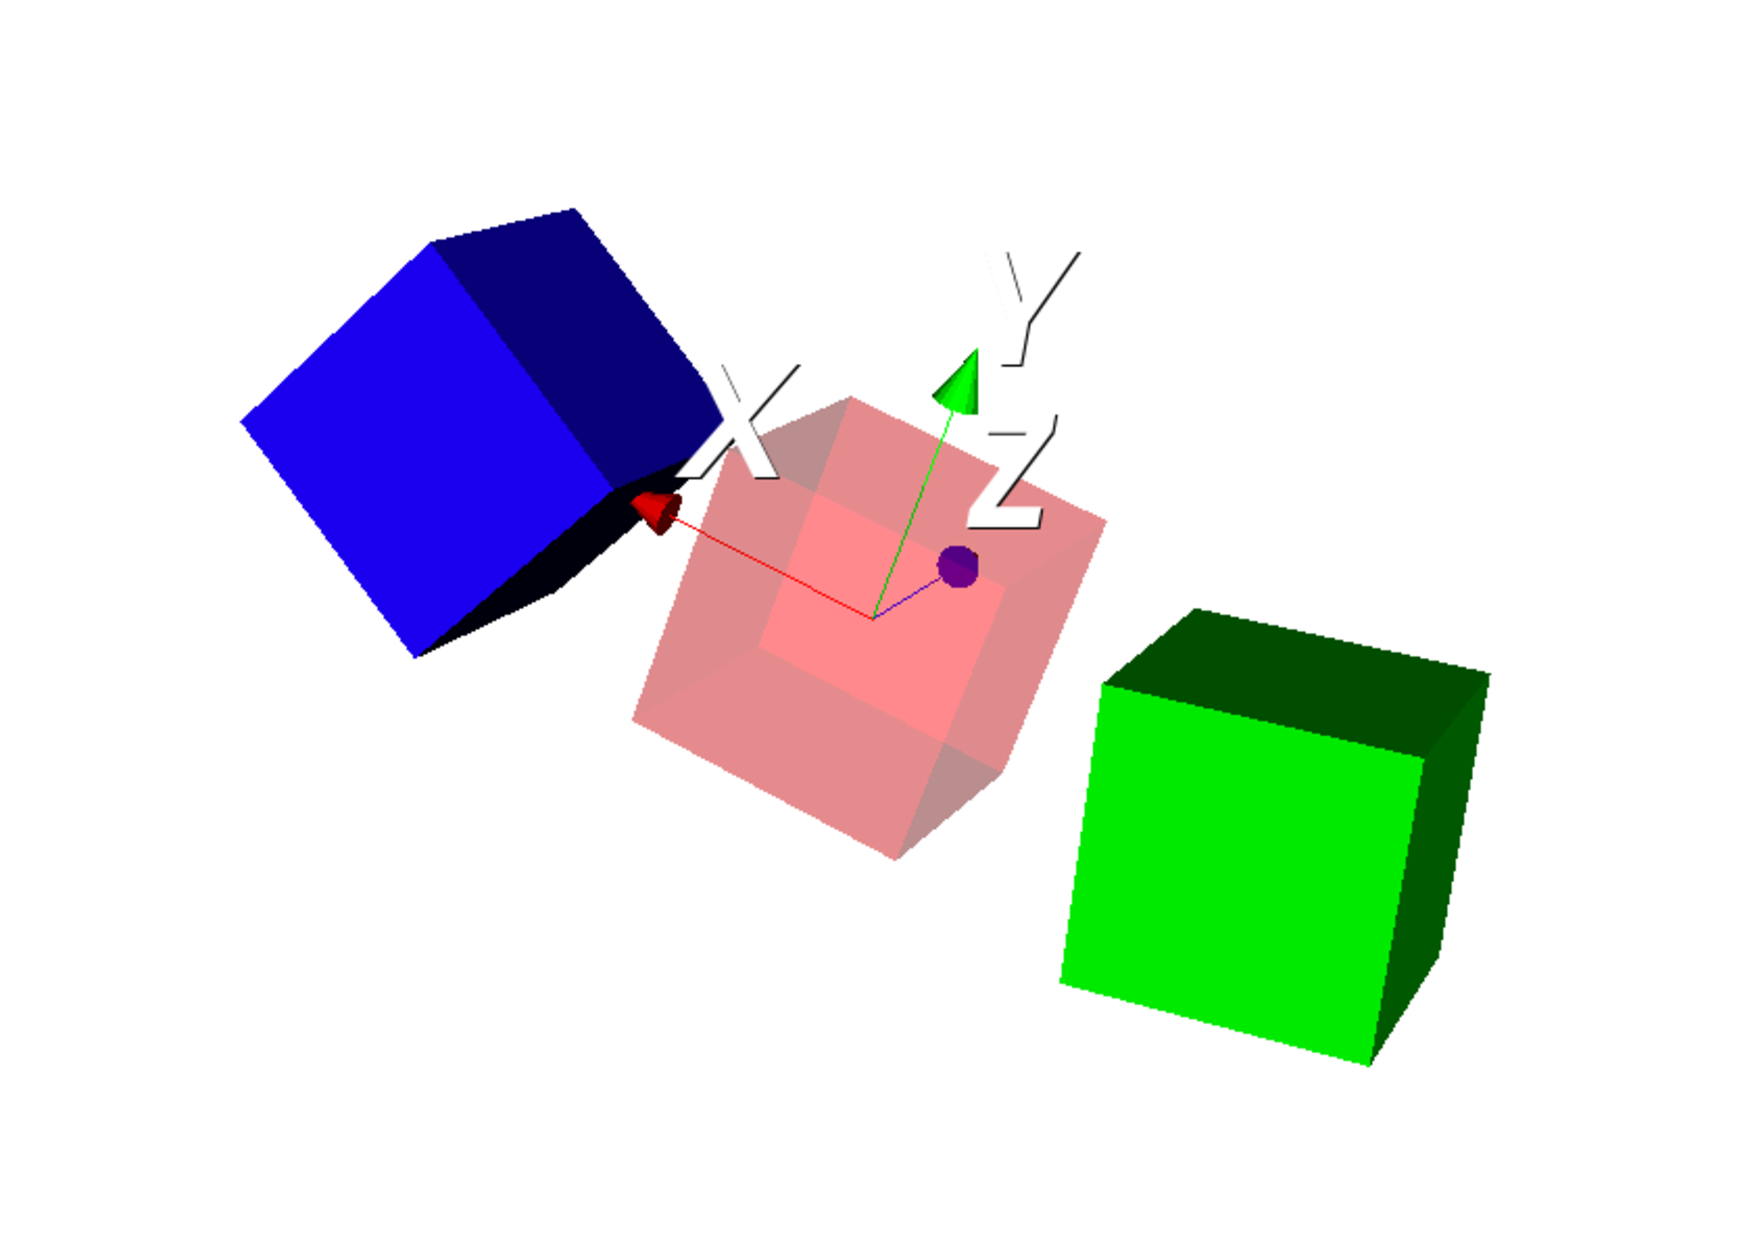
\includegraphics[width=7cm]{./diagrams/rapidModelling.pdf}
\caption{VTK visualisation output from code example XXX.}
\label{fig:rapidModellingExample}
\end{center}
\end{figure}
Significantly more complex geometries can be developed using a structure similar to that shown in code listing XXX.  

\section{CAD to Geant4 conversion }
STEP and IGES files can be loaded into pyg4ometry, via an interface based on FreeCAD. FreeCAD is an open source CAD/CAM program, which in turn 
is based on OpenCASCADE. A STEP CAD file could be considered as a hierarchical tree of {\it part assemblies} and {\it part features}, where a part assembly is a 
collection of part features. A part feature can be used to create  a triangular mesh which can used to create a pyg4ometry tessellated solid. Assignment of materials 
and visualisation attributes. 

\section{FLUKA to Geant4 conversion}
FLUKA geometry is based upon a limited set of primitive volumes which can be combined using logical operations. Many FLUKA primitives are infinite in extent, so 
to emulate FLUKA geometry construction large but finite extent Geant4 primitive solids are used. Table \ref{tab:Fluka2Geant4} shows the mapping between FLUKA and Geant4 objects.
An ANTLR based expression parser is used to load and comprehend the FLUKA input syntax, an example is shown in XXX. Each FLUKA body is matched to a Geant4 
solid and a FLUKA region is represented by a Geant4 CSG tree is formed using the pyg4ometry classes. 

\begin{table}[hbt!]
\centering
\begin{tabular}{|l|l|} \hline
FLUKA body							& pyg4ometry class 		\\ \hline
RPP 	(Rectangular parallelepiped)			& Box				\\
BOX	(General rectangular parallelepiped)		& Box				\\
SPH 	(Sphere)							& Orb				\\
RCC (Right circular cylinder)				& Cone				\\
REC (Right elliptical cylinder)				& EllipticalTube			\\
TRC (Truncated Right Angle Cone)			& Cone				\\
ELL (Ellipsoid of Revolution) 				& Ellipsoid				\\
WED/RAW (Right Angle Wedge)			& ExtrudedSolid		\\
ARB	(Arbitrary Convex Polyhedron)			& TessellatedSolid		\\
XYP 	($X$-$Y$ Infinite half-space)			& Box				\\
XZP 	($X$-$Z$ Infinite half-space)			& Box				\\
YZP 	($Y$-$Z$ Infinite half-space)			& Box				\\
PLA (Generic infinite half-space)			& Box				\\
XCC ($X$-axis Infinite Circular Cylinder)		& Tubs				\\
YCC ($Y$-axis Infinite Circular Cylinder)		& Tubs				\\
ZCC 	($Z$-axis Infinite Circular Cylinder)		& Tubs				\\
XEC 	($X$-axis Infinite Elliptical Cylinder)		& EllipticalTube			\\
YEC 	($Y$-axis Infinite Elliptical Cylinder)		& EllipticalTube			\\
ZEC ($Z$-axis Infinite Elliptical Cylinder)		& EllipticalTube			\\
QUA (Quadric surface) 					& TessellatedSolid		\\ \hline
\end{tabular}
\caption{FLUKA geometry directives pyg4ometry classes.} \label{tab:Fluka2Geant4}
\end{table}

\begin{enumerate} 
\item length safety
\item infinite planes
\item disjoint unions 
\end{enumerate} 

\section{Geant4 to FLUKA conversion}
It is relatively straight forward to convert Geant4 geometry to FLUKA. Each of the Geant4 solids can be mapped to a FLUKA CSG region.
Some solids in Geant4 directly map to a FLUKA body, others need a construction of a simple FLUKA CSG tree. 


\begin{table}[hbt!]
\centering
\begin{tabular}{| l | l | } \hline
Geant4 solid			& FLUKA region constuction		\\ \hline
Box					& +2 XYP + 2 XZP + 2 YZP 		\\
Tube					& +ZCC - 2 XYP	 			\\
CutTube				& +ZCC - 2 PLA				\\
Cone				& +TRC -TRC - WED			\\
Para					& +ARB						\\
Trd					& +ARB						\\
Trap					& +ARB						\\
Sphere				& +SPH - SPH  - WED - TRC		\\
Orb					& +SPH						\\
Torus				& +$N$ ZCC  - $N$ PLA			\\
Polycone				& +$N$ ARB					\\
GenericPolycone		& +$N$ ARB					\\
Polyhedra				& +$N$ ARB					\\
Eltube				& +ZEC  - 2 XYP				\\
Ellipsoid				& +ELL - 2 XYP		 			\\
Elcone				& +QUA - 2 XYP				\\
Paraboloid			& +QUA - 2 XYP				\\
Hype					& +QUA - 2 XYP				\\
Tet					& +ARB						\\
Xtru					& +$N$ ARB					\\
TwistedBox			& +$N$ ARB					\\
TwistedTtap			& +$N$ ARB					\\
TwistedTrd			& +$N$ ARB				 	\\
TwistedTube			& +$N$ ARB					\\
Arb8					& +ARB						\\
Tessellated			& N/A					 	\\
Union				& | zone1 | zone2				\\
Subtraction			& +zone1 -zone2				\\
Intersection			& +zone1 +zone2				\\
MultiUnion			& | zone1 | zone2 | zone3 | ...	\\
ScaledSolid			& geant4.solid.ScaledSolid		\\ \hline				
\end{tabular}
\caption{GDML/Geant4 solids and the mapping to FLUKA bodies}
\end{table}

\section{Interesting use cases}
pyg4ometry is designed to be as flexible as possible and offer the user a wide range of usage styles and workflows. The following sections describe a selection of 
possible applications.

\subsection{Mixing geometry sources}
It is possible to mix different geometries from STL, STEP, GDML and FLUKA in single GDML file for use in Geant4 and ROOT. 

\subsection{Editing existing models}
Often existing CAD models have either missing details or too many details. Examples of too potentially superfluous detail are gaskets and bolts 

\subsection{Overlap checking in geometry}
Often small errors in geometry cause unexpected RT code behaviour.  


\section{Performance of converted geometry in Geant4}
Clearly for Geant4 geometry defined in pyg4ometry the performance is exactly the same as it the geometry was specified in C++ and linked against the Geant4
libraries. A comparison of the performance of converted CAD or FLUKA geometry compared with native Geant4 solids is required so a user can optimise the available
computing resources against the human resources (required to convert geometry). BDSIM is used to load the pyg4ometry generated files  and run basic simulations where 
high energy particles are   

\section{Conclusions}
The authors believe that tools to quickly create, either ab-initio or by conversion geometry usable in particle transport Monte Carlo programmes will save significant 
amounts of user effort and ultimately yield more accurate simulations. Pyg4ometry is a relatively complete implementation of a geometry creation tool, whilst heavily 
internally based on Geant4 and GDML can have utility for users of all RT codes. Pyg4ometry can clearly be extended to other formats or applications. As for applications,
examples include  the  generation triangular mesh structures for GPU accelerated photon tracking in liquid noble  dark matter detectors and geometries for event visualisation. 
Although not implemented in the current version, a C++ output writer can be quickly implemented to generate geometry which can be compiled into a Geant4 application. 

%% The Appendices part is started with the command \appendix;
%% appendix sections are then done as normal sections
%% \appendix

%% \section{}
%% \label{}

%% References
%%
%% Following citation commands can be used in the body text:
%% Usage of \cite is as follows:
%%   \cite{key}         ==>>  [#]
%%   \cite[chap. 2]{key} ==>> [#, chap. 2]
%%

%% References with bibTeX database:

\bibliographystyle{elsarticle-num}
\bibliography{pyg4ometry}
%% Authors are advised to submit their bibtex database files. They are
%% requested to list a bibtex style file in the manuscript if they do
%% not want to use elsarticle-num.bst.

%% References without bibTeX database:

% \begin{thebibliography}{00}

%% \bibitem must have the following form:
%%   \bibitem{key}...
%%

% \bibitem{}

% \end{thebibliography}


\end{document}

%%
%% End of file 